\documentclass[12pt, a4paper, oneside]{ctexart}
\usepackage{amsmath, amsthm, amssymb, appendix, bm, graphicx, hyperref, mathrsfs}
\usepackage{fontspec}
\usepackage{listings}
\usepackage{color}
\usepackage{xcolor}
\definecolor{dkgreen}{rgb}{0,0.6,0}
\definecolor{gray}{rgb}{0.5,0.5,0.5}
\definecolor{mauve}{rgb}{0.58,0,0.82}
\lstset{frame=tb,
     language=Java,
     aboveskip=3mm,
     belowskip=3mm,
     showstringspaces=false,
     columns=flexible,
     basicstyle = \ttfamily\small,
     numbers=left,
     numberstyle=\tiny\color{gray},
     keywordstyle=\color{blue},
     commentstyle=\color{dkgreen},
     stringstyle=\color{mauve},
     breaklines=true,
     breakatwhitespace=true,
     tabsize=4
}

\CTEXsetup[format={\Large\bfseries}]{section}

\title{\textbf{测试计划}}
\author{第25组}
\date{\today}

\begin{document}


\maketitle
\section{概述}
\subsection{测试需求}
本次作业要求使用白盒测试。我们选择了一个红黑树的java实现作为测试对象,使用Junit框架进行单元测试。

\subsection{任务分配}
本小组为四人小组,任务分配为:

\subsection{总体思路}
由于被测软件有很多方法是private的方法,\textbf{为了使得测试方便,我们将所有方法全部改成public}。原软件的所有public接口,写在RBTree.java顶部的注释中。

首先, colorOf 和 parentOf 等简单的accessor方法,以及 setColor 等简单的set方法,可以看做类似于宏,不需要进行单元测试,\textbf{只要其他方法的单元测试通过了,这些方法必然被覆盖到}。

因此,先测试各个查找方法。然后在测试修改树结构有关的方法时,首先需要测试左旋、右旋方法,然后测试重新平衡方法。最后再测试插入、删除方法。在本测试计划中,以下各个的单元测试是按照顺序进行的。


\section{对search方法的测试}

search方法代码如下。在实际使用中,search一定是从根节点开始查找,因此两个方法可以合并测试。

\begin{lstlisting} [language = Java]
public RBTNode<T> search(RBTNode<T> x, T key) {
    if (x==null)
        return x;

    int cmp = key.compareTo(x.key);
    if (cmp < 0)
        return search(x.left, key);
    else if (cmp > 0)
        return search(x.right, key);
    else
        return x;
}

public RBTNode<T> search(T key) {
    return search(mRoot, key);
}
\end{lstlisting}

各个节点的定义如下

\newpage
\begin{table}[!h]
    \begin{tabular}{|l|l|}
    \hline
    代码行 & DD路径名称\\ \hline
    1 & A\\ \hline
    2 & B\\ \hline
    3 & C \\ \hline
    5 & D \\ \hline
    6 & E \\ \hline
    7 & F \\ \hline
    8 & G \\ \hline
    9 & H \\ \hline
    10-11 & I \\ \hline
    12 & J \\ \hline
    12-end & K \\ \hline
    \end{tabular}
\end{table}

其中,12-end描述的行为是在接收函数返回值并退出。

\subsection{DD路径分析和数据流分析}

递归是一种特殊的循环。因此可以分析DD路径如下

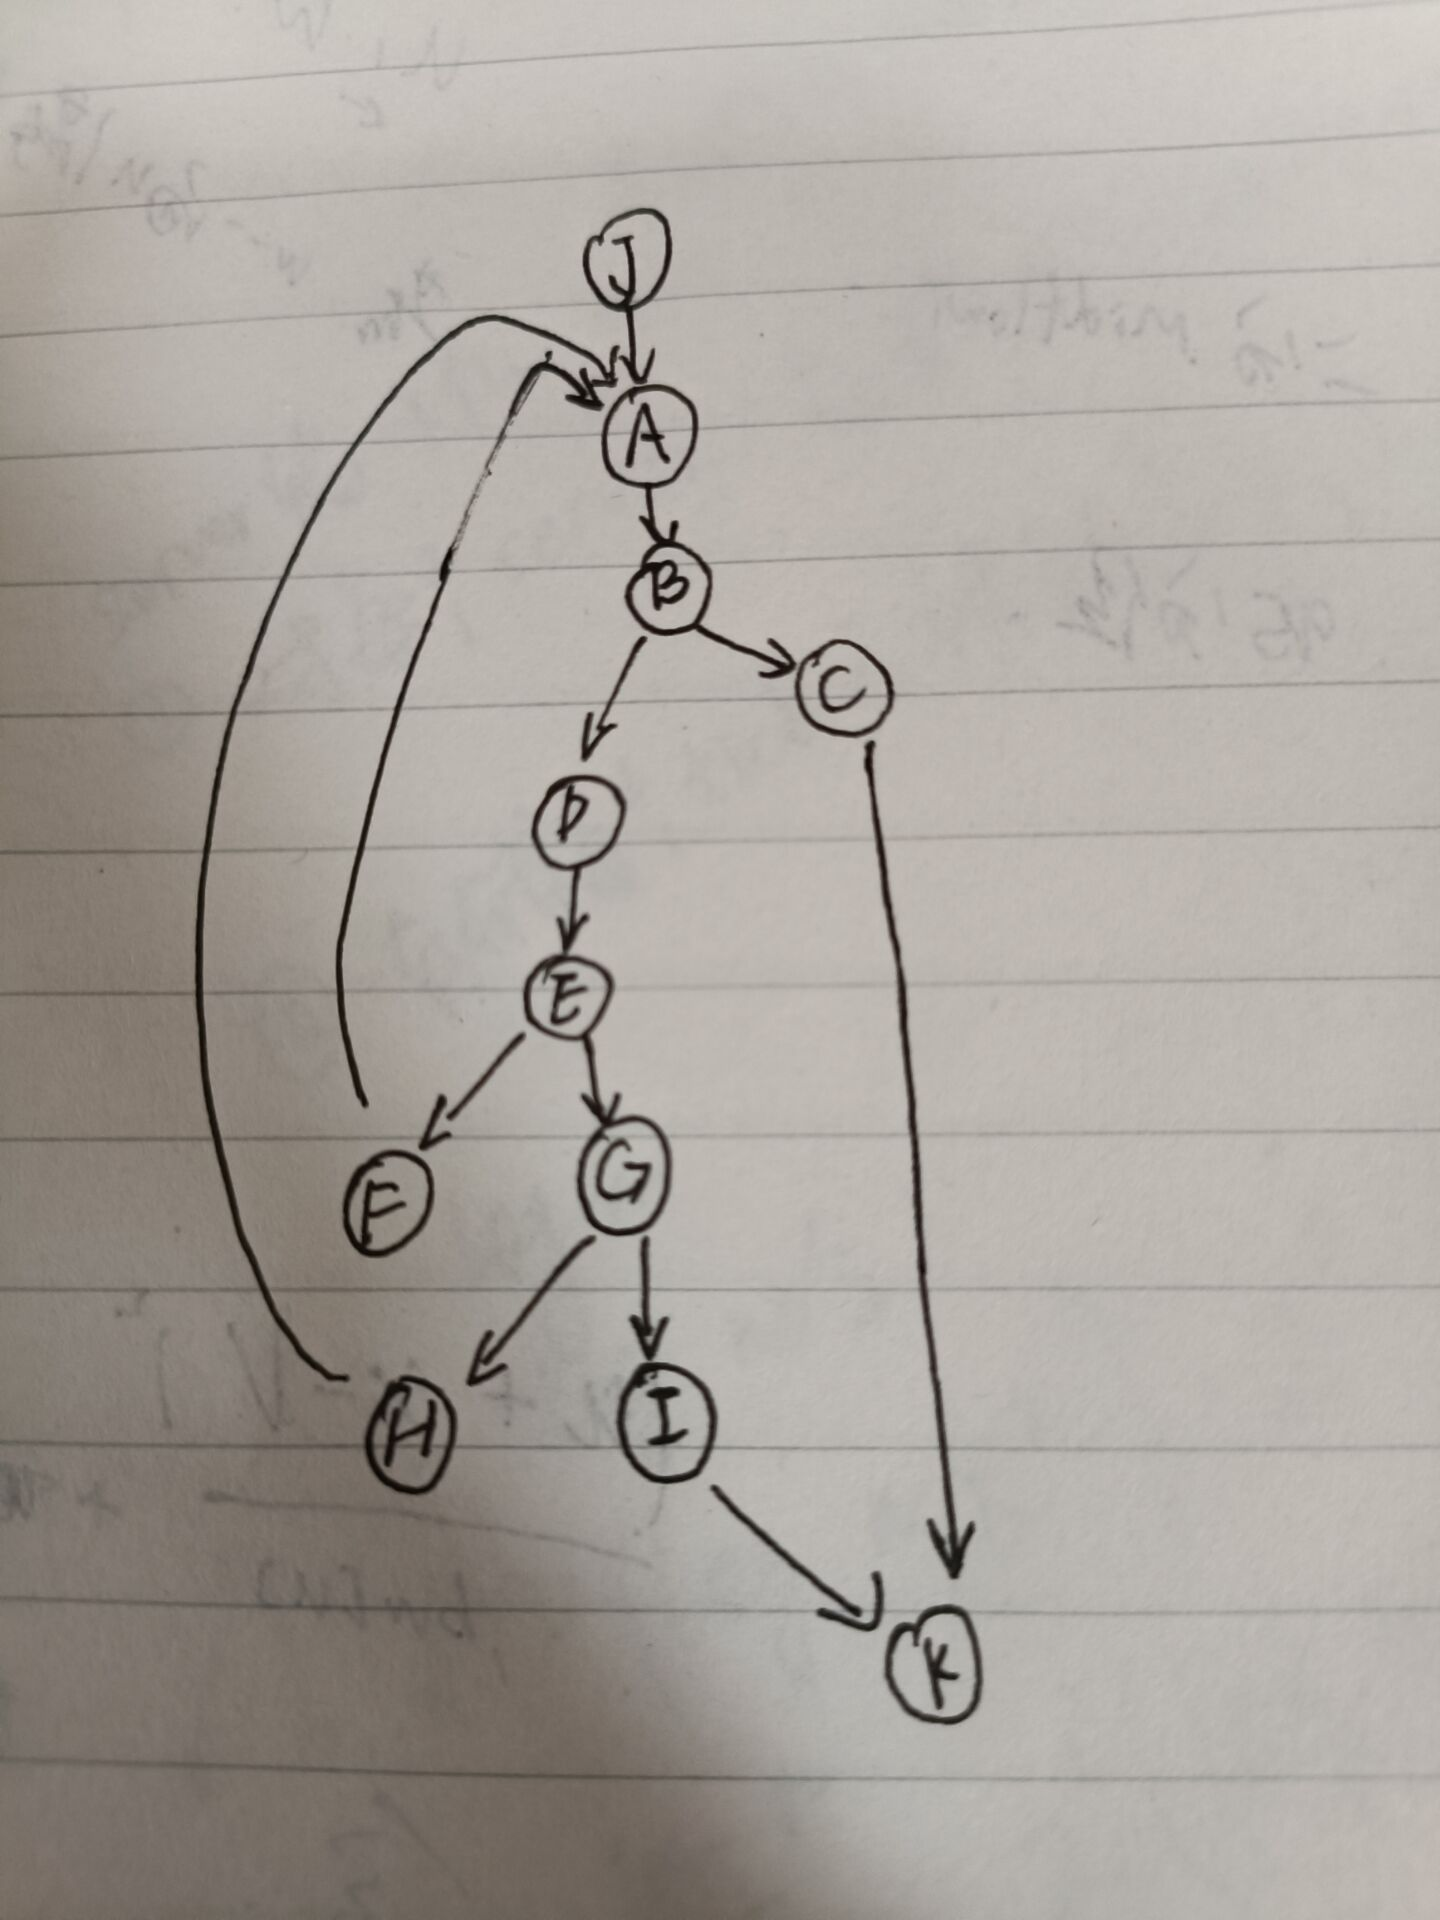
\includegraphics[scale=0.2]{screenshots/DD-search.jpg}

数据流分析如下

\begin{table}[!h]
    \begin{tabular}{|l|l|l|}
    \hline
    变量名 & 定义节点 & 使用节点 \\ \hline
    x & A & B C D F H I\\ \hline
    key & A & F H \\ \hline
    cmp & D & E G \\ \hline
    \end{tabular}
\end{table}

在这个方法的单元测试中,使用数据流分析的结果设计用例,覆盖指标采用\textbf{全使用准则}。
因此,测试用例的执行路径集合,需要覆盖以下路径:A-B, A-C, A-D, A-F, A-H, A-I, D-E, D-G.

\subsection{用例设计}

用例的设计代码如下。首先构造一个红黑树,然后依次查询权值为5, 6, 114514的节点。红黑树的形态如下图所示:

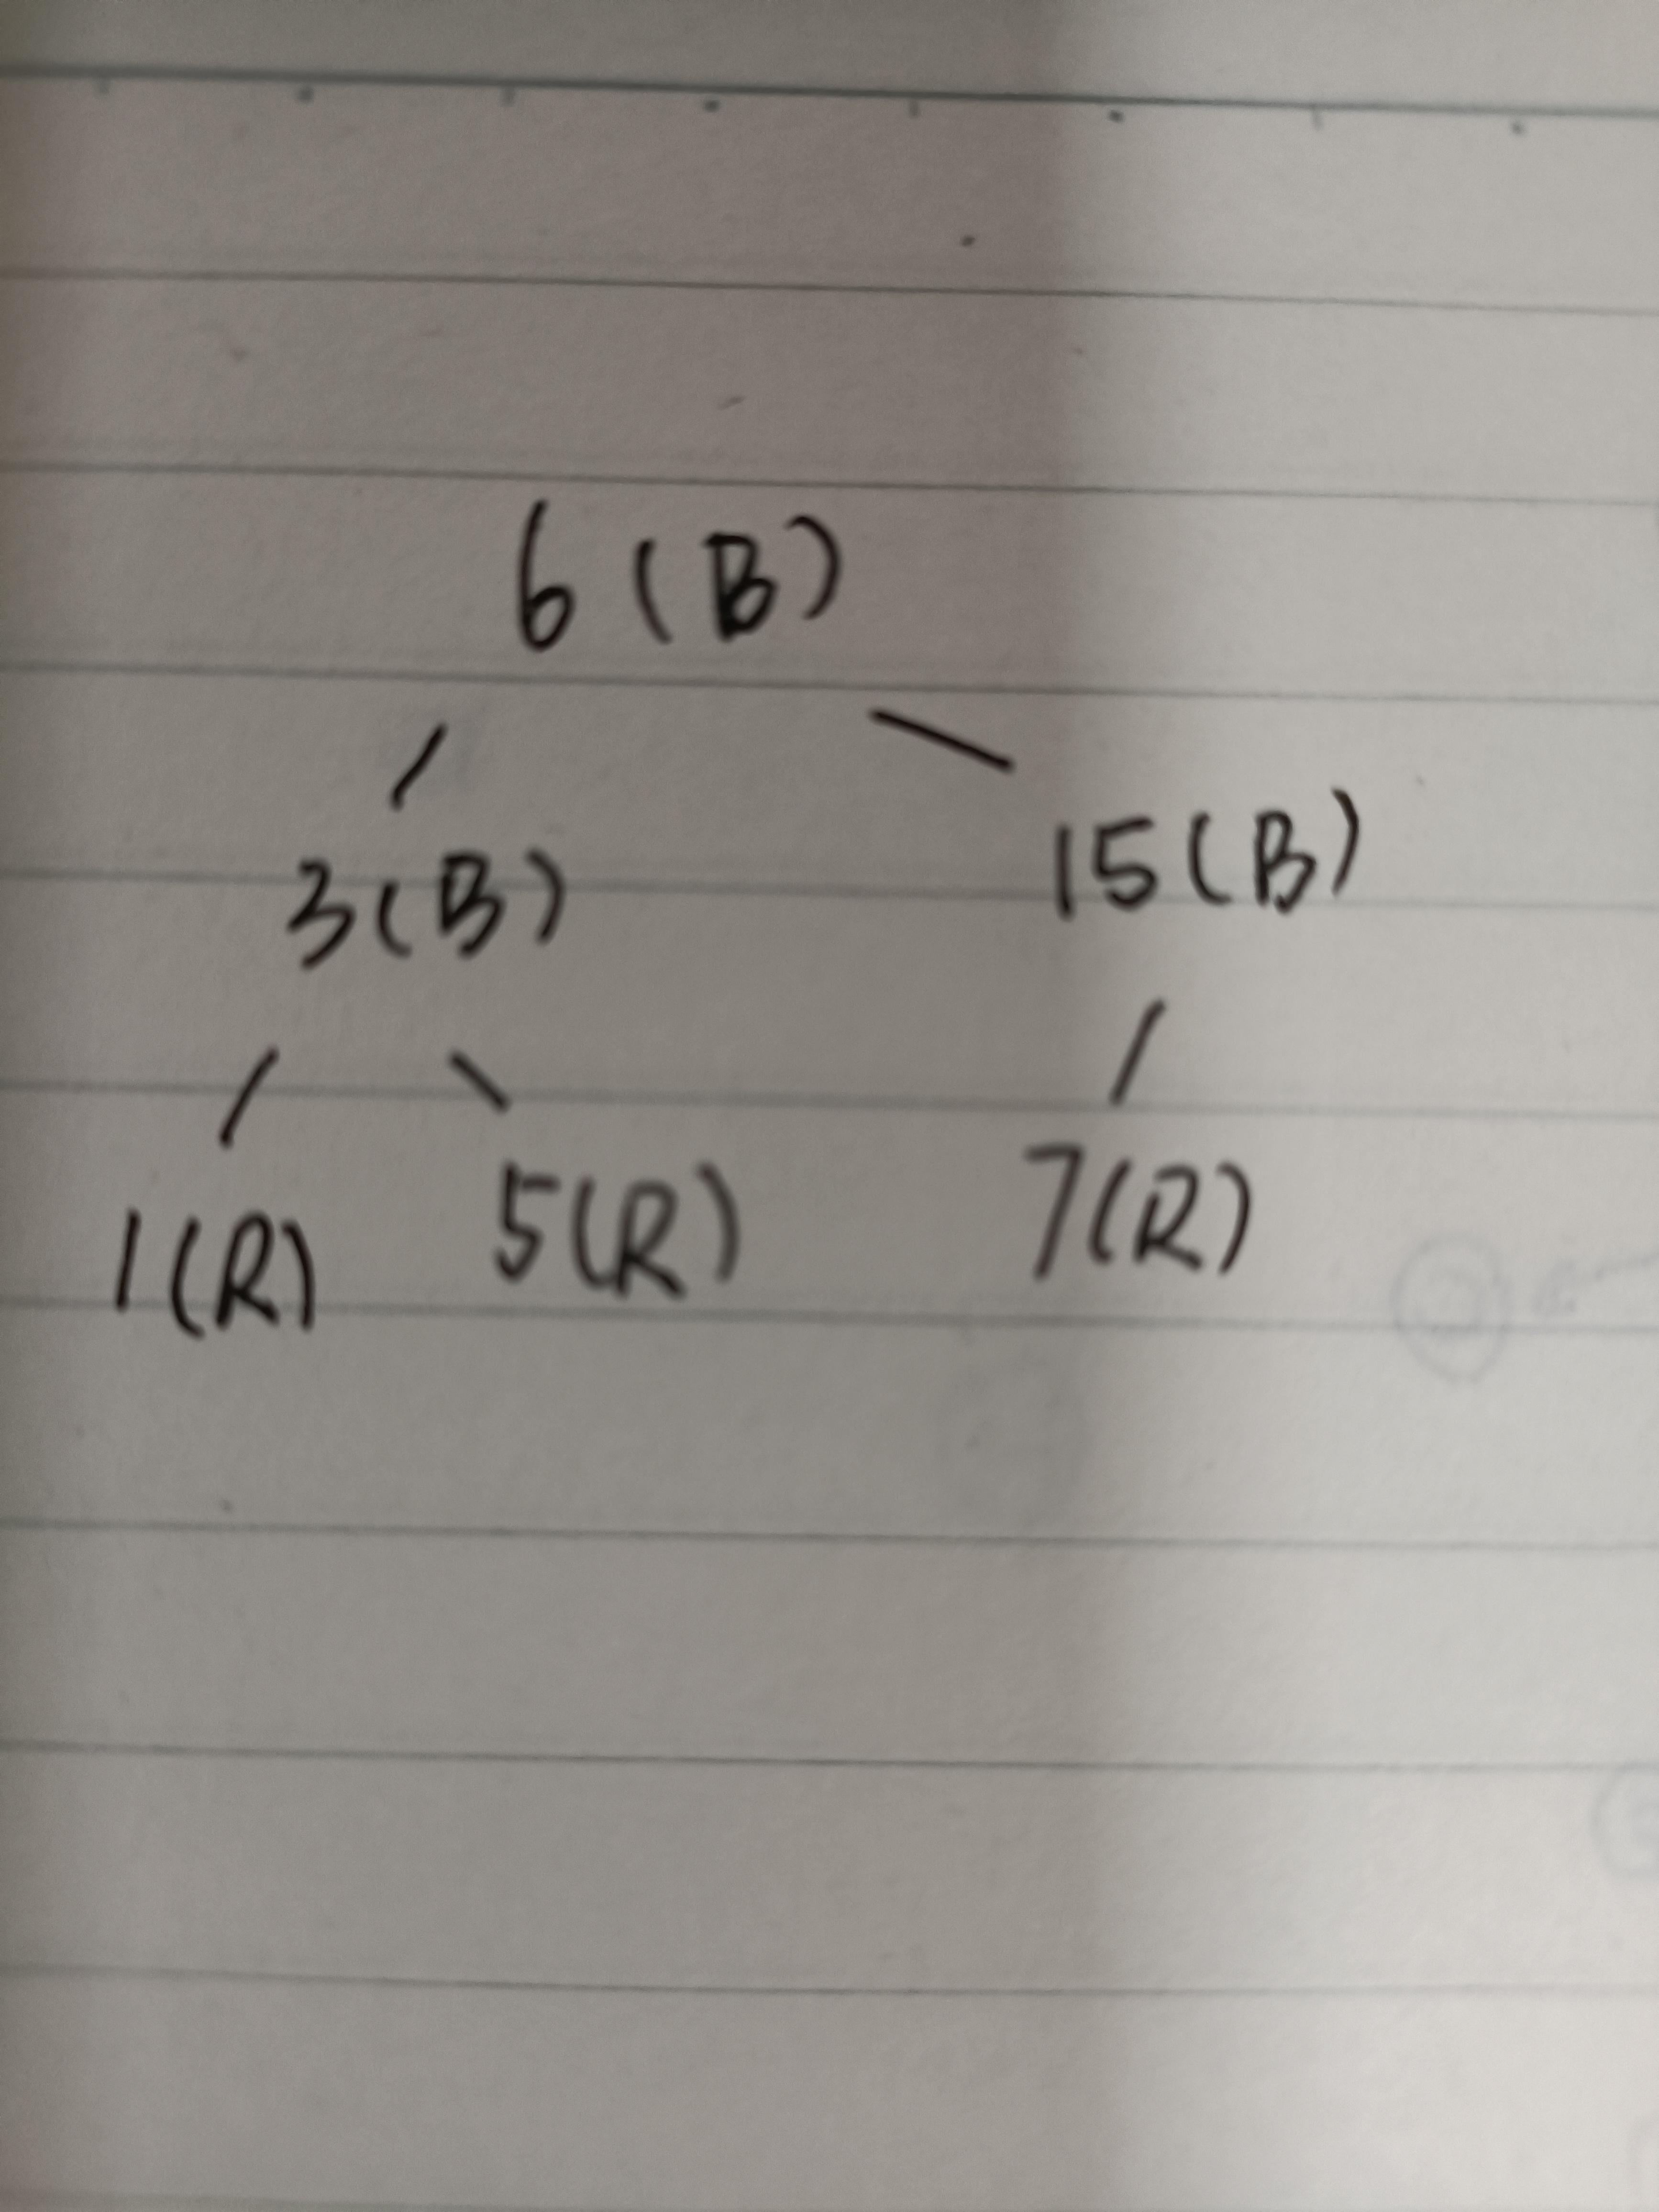
\includegraphics[scale=0.07]{screenshots/RBT-search.jpg}

\begin{lstlisting} [language = Java]
@Test
void search() {
    tree = new RBTree<>();
    tree.mRoot = new RBTNode<>(6, true,null,null,null);
    RBTNode<Integer> node1 = new RBTNode<>(3, true, null, null, null);
    RBTNode<Integer> node2 = new RBTNode<>(1, false, null, null, null);
    RBTNode<Integer> node3 = new RBTNode<>(5, false, null, null, null);
    RBTNode<Integer> node4 = new RBTNode<>(15, true, null, null, null);
    RBTNode<Integer> node5 = new RBTNode<>(7, false, null, null, null);

    tree.mRoot.left = node1; tree.mRoot.right = node4;
    node1.parent = tree.mRoot; node1.left = node2; node1.right = node3;
    node2.parent = node1;
    node3.parent = node1;
    node4.parent = tree.mRoot; node4.left = node5;
    node5.parent = node4;

    RBTNode<Integer> node = tree.search(6);
    assertEquals(node, tree.mRoot);
    node = tree.search(5);
    assertEquals(node, node3);
    node = tree.search(114514);
    assertNull(node);
}
\end{lstlisting}

\end{document}
